\section{Experiments}
This section will give an explanation on the two experiments performed using the framework.
The first part of the section will describe the experimental setup common to the two experiments which was used.
The two subsection will dive in:
\begin{itemize}
	\item MRAM vs SRAM layer 2 memory
	\item SRAM clock exploration on layer 2 memory
	\item Reference to the paper for MRAM specs~\cite{8310393}
\end{itemize}

\subsection{MRAM vs SRAM layer 2 memory}

\begin{figure}[tb] 
\centering
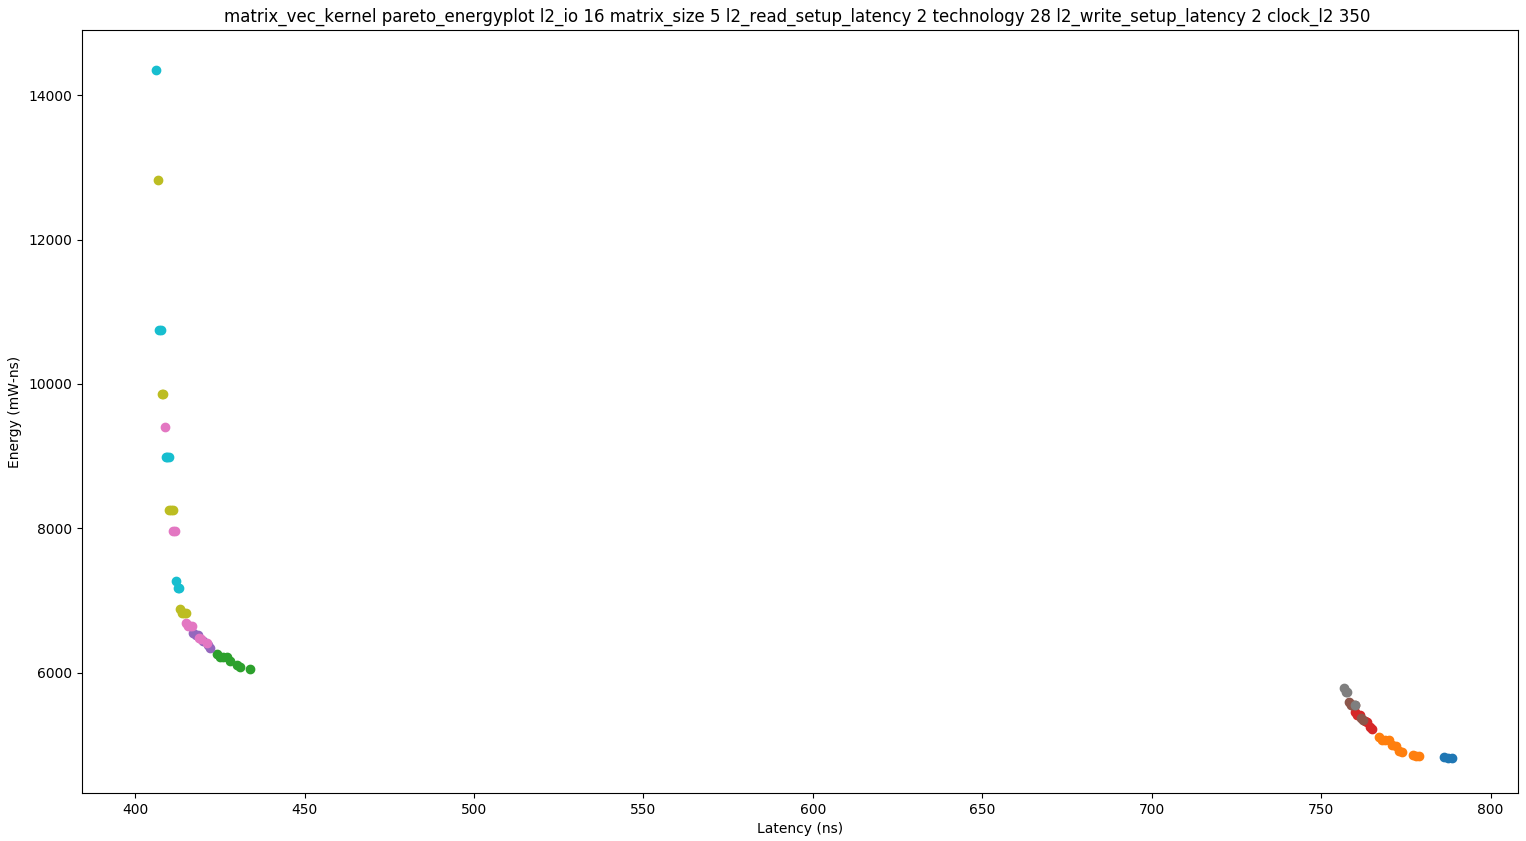
\includegraphics[width=\columnwidth]{images/sram_mram_matrix_vec_energy_pareto_2.png}
\caption{\small Energy Pareto Graph, each point corresponds to an architecture generated by the framework. Different colors are associated each initial configuration file. The cluster of archiectures on the left side of this graph are using an SRAM memory in Layer 2, the cluster on the right uses an MRAM memory. }
\label{fig:sram_mram_energy_graph}
\end{figure}

Figure~\ref{fig:sram_mram_energy_graph} shows the pareto points in the energy-latency graph.
\begin{itemize}
\item The most energy efficient MRAM architecture consumes 20.5\% less energy than the SRAM counterpart.
\item The most energy efficient MRAM architecture takes 81.5\% more time than the SRAM counterpart.
\end{itemize}

\subsection{MRAM vs SRAM layer 2 memory}

\begin{figure}[tb] 
\centering
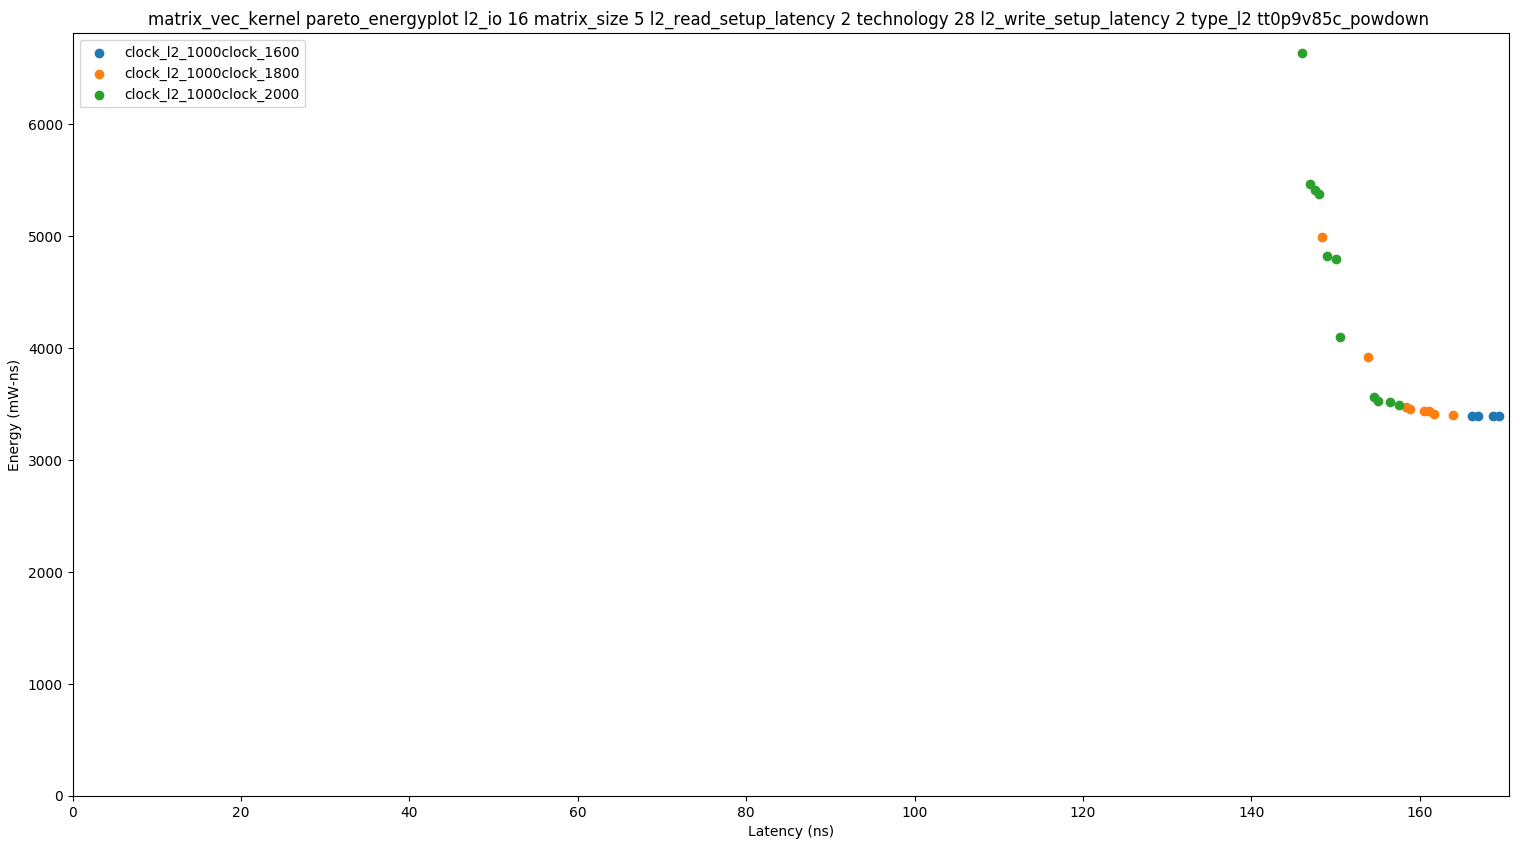
\includegraphics[width=\columnwidth]{images/sram_clocks_matrix_vec_5_energy_pareto.png}
\caption{\small Energy Pareto Graph, each point corresponds to an architecture generated by the framework. Different colors are associated each initial configuration file.}
\label{fig:srams_energy_graph}
\end{figure}

Figure~\ref{fig:srams_energy_graph} shows the pareto points in the energy-latency graph.
\begin{itemize}
	\item The most energy efficient designs are obtained using the highest possible clock for the Layer 2 SRAM memory (1GHz).
	\item The architecture consuming less energy has a Layer 2 clock frequency of 1GHz and a Layer 1 clock frequency of 1600 MHz.
\end{itemize}


